\chapter{插值}\label{chap:appendix-c}

\begin{note}[动机]\label{note:appendix-c-1}
偏微分方程的变分形式以 Sobolev 空间中的函数为对象.求解这类方程时,需用有限维空间——即有限元空间——中的函数通过 Ritz 方法作近似.Sobolev 空间中任意函数的最佳有限元逼近误差,是有限元误差上界中的一个因子,例如 Céa 引理\hyperref[lem:cea]{(B.12)} 所示.本附录研究有限元空间的逼近质量,并证明函数插值误差估计.这些估计给出了最佳逼近误差的上界,也可作为有限元误差估计中的因子.
\end{note}

\section{Sobolev 空间中的多项式插值}\label{sec:appendix-c-1}

\begin{lemma}[积分条件唯一确定多项式]\label{lem:appendix-c-2}
设 $\Omega\subset\mathbb R^d$ 是具有 Lipschitz 边界的有界区域,给定
$m\in\mathbb N\cup\{0\}$.对每个满足 $|\alpha|\le m$ 的多重指标 $\alpha$,给定一个数 $a_\alpha\in\mathbb R$.则存在唯一的多项式 $p\in P_m(\Omega)$,使得
\begin{equation}\label{eq:appendix-c-1}
 \int_\Omega \partial^\alpha p(\bm x)\,\mathrm d\bm x
 =a_\alpha,\qquad |\alpha|\le m.
\end{equation}
\end{lemma}

\begin{proof}
任取 $p\in P_m(\Omega)$,可将其写为
\[
 p(\bm x)=\sum_{|\beta|\le m}b_\beta\bm x^\beta.
\]
将此表示代入式\hyperref[eq:appendix-c-1]{(C.1)},得到线性方程组
$M\bm b=\bm a$,其中
\[
 M=(M_{\alpha\beta}),\qquad
 M_{\alpha\beta}=\int_\Omega\partial^\alpha\bm x^\beta\,\mathrm d\bm x,
 \qquad \bm b=(b_\beta),\quad \bm a=(a_\alpha),
\]
指标满足 $|\alpha|,|\beta|\le m$.由于 $M$ 是方阵,该方程组有唯一解,当且仅当 $M$ 非奇异.

反设 $M$ 奇异,则对应的齐次方程组存在非零解.也就是说,存在非零多项式 $q\in P_m(\Omega)$,使得
\[
 \int_\Omega\partial^\alpha q(\bm x)\,\mathrm d\bm x=0,
 \qquad |\alpha|\le m.
\]
将 $q$ 写为 $q(\bm x)=\sum_{|\beta|\le m}c_\beta\bm x^\beta$.选取一个满足 $c_\beta\ne0$ 且 $|\beta|$ 最大的指标 $\beta$.于是
$\partial^\beta q(\bm x)=C c_\beta$ 是非零常数,其中 $C>0$ 来自多项式的求导规则.这与 $\partial^\beta q$ 的积分为零矛盾.
\end{proof}

\begin{lemma}[Poincaré 型不等式]\label{lem:appendix-c-3}
记 $D^k v(\bm x)$ 为函数 $v(\bm x)$ 的 $k$ 阶全导数,其中
$k\in\mathbb N\cup\{0\}$;例如,$k=1$ 时为梯度.设 $\Omega$ 是凸集,且包含在半径为 $R$ 的球内.令 $l\in\mathbb N\cup\{0\}$、$k\le l$,并令 $p\in[1,\infty)$.假设 $v\in W^{l,p}(\Omega)$ 满足
\[
 \int_\Omega\partial^\alpha v(\bm x)\,\mathrm d\bm x=0,
 \qquad |\alpha|\le l-1.
\]
则有估计
\[
 \|D^k v\|_{L^p(\Omega)}
 \le CR^{l-k}\|D^l v\|_{L^p(\Omega)},
\]
其中常数 $C$ 与 $\Omega$ 和 $v$ 无关.
\end{lemma}

\begin{proof}
当 $k=l$ 时结论显然.此外,只需证明 $k=0$、$l=1$ 的情形;一般情形可将该结果依次应用于 $\partial^\alpha v$.

由于 $\Omega$ 是凸集,可将积分中值定理写为
\[
 v(\bm x)-v(\bm y)
 =\int_0^1\nabla v(t\bm x+(1-t)\bm y)
   \cdot(\bm x-\bm y)\,\mathrm dt,
 \qquad \bm x,\bm y\in\Omega.
\]
对 $\bm y$ 积分,得到
\[
 v(\bm x)\int_\Omega\mathrm d\bm y
 -\int_\Omega v(\bm y)\,\mathrm d\bm y
 =\int_\Omega\int_0^1
   \nabla v(t\bm x+(1-t)\bm y)\cdot(\bm x-\bm y)
   \,\mathrm dt\,\mathrm d\bm y.
\]
由零均值条件,左端第二项为零.因此
\[
 v(\bm x)=\frac1{|\Omega|}
 \int_\Omega\int_0^1
   \nabla v(t\bm x+(1-t)\bm y)\cdot(\bm x-\bm y)
   \,\mathrm dt\,\mathrm d\bm y.
\]
取绝对值,并利用积分绝对值不超过绝对值的积分、向量 Cauchy--Schwarz 不等式\hyperref[eq:appendix-a-2]{(A.2)},以及
$\|\bm x-\bm y\|_2\le2R$,得
\begin{equation}\label{eq:appendix-c-2}
\begin{aligned}
 |v(\bm x)|
 &=\frac1{|\Omega|}\left|
   \int_\Omega\int_0^1
    \nabla v(t\bm x+(1-t)\bm y)\cdot(\bm x-\bm y)
    \,\mathrm dt\,\mathrm d\bm y\right|\\
 &\le\frac1{|\Omega|}\int_\Omega\int_0^1
   \left|\nabla v(t\bm x+(1-t)\bm y)\cdot(\bm x-\bm y)\right|
   \,\mathrm dt\,\mathrm d\bm y\\
 &\le\frac{2R}{|\Omega|}\int_\Omega\int_0^1
   \|\nabla v(t\bm x+(1-t)\bm y)\|_2
   \,\mathrm dt\,\mathrm d\bm y.
\end{aligned}
\end{equation}

将式\hyperref[eq:appendix-c-2]{(C.2)} 两边取 $p$ 次方并对 $\bm x$ 积分.利用 Hölder 不等式\hyperref[eq:appendix-a-9]{(A.9)},其中 $p^{-1}+q^{-1}=1$,可得
\[
\begin{aligned}
 \int_\Omega|v(\bm x)|^p\,\mathrm d\bm x
 &\le\frac{CR^p}{|\Omega|^p}
 \int_\Omega\left[
   \int_\Omega\int_0^1
    \|\nabla v(t\bm x+(1-t)\bm y)\|_2
    \,\mathrm dt\,\mathrm d\bm y
 \right]^p\mathrm d\bm x\\
 &\le\frac{CR^p}{|\Omega|^p}
 \int_\Omega
  \left[\int_\Omega\int_0^1 1^q\,\mathrm dt\,\mathrm d\bm y\right]^{p/q}
  \\
  &\quad\times\left[\int_\Omega\int_0^1
   \|\nabla v(t\bm x+(1-t)\bm y)\|_2^p
   \,\mathrm dt\,\mathrm d\bm y\right]\mathrm d\bm x\\
 &=\frac{CR^p}{|\Omega|}
  \int_\Omega\int_\Omega\int_0^1\\
  &\quad\|\nabla v(t\bm x+(1-t)\bm y)\|_2^p
   \,\mathrm dt\,\mathrm d\bm y\,\mathrm d\bm x.
\end{aligned}
\]
利用 Fubini 定理交换积分次序,得到
\[
 \int_\Omega|v(\bm x)|^p\,\mathrm d\bm x
 \le\frac{CR^p}{|\Omega|}\int_0^1\int_\Omega
   \left[\int_\Omega
    \|\nabla v(t\bm x+(1-t)\bm y)\|_2^p
    \,\mathrm d\bm y\right]
   \,\mathrm d\bm x\,\mathrm dt.
\]
由一维积分中值定理,存在 $t_0\in[0,1]$,使得
\[
 \int_\Omega|v(\bm x)|^p\,\mathrm d\bm x
 \le\frac{CR^p}{|\Omega|}\int_\Omega
   \left[\int_\Omega
    \|\nabla v(t_0\bm x+(1-t_0)\bm y)\|_2^p
    \,\mathrm d\bm y\right]
   \,\mathrm d\bm x.
\]
将 $\|\nabla v(\bm x)\|_2^p$ 零延拓到 $\mathbb R^d$,仍用同一记号表示.于是
\begin{equation}\label{eq:appendix-c-3}
 \int_\Omega|v(\bm x)|^p\,\mathrm d\bm x
 \le\frac{CR^p}{|\Omega|}\int_\Omega
   \left[\int_{\mathbb R^d}
    \|\nabla v(t_0\bm x+(1-t_0)\bm y)\|_2^p
    \,\mathrm d\bm y\right]
   \,\mathrm d\bm x.
\end{equation}

设 $t_0\in[0,1/2]$.由于积分区域是 $\mathbb R^d$,作变量代换
$t_0\bm x+(1-t_0)\bm y=\bm z$,可得
\[
 \int_{\mathbb R^d}
   \|\nabla v(t_0\bm x+(1-t_0)\bm y)\|_2^p\,\mathrm d\bm y
 =\frac1{(1-t_0)^d}\int_{\mathbb R^d}\|\nabla v(\bm z)\|_2^p\,\mathrm d\bm z
 \le2^d\|\nabla v\|_{L^p(\Omega)}^p.
\]
此处 $d$ 次幂来自 $d$ 维变量代换.将该估计代入式\hyperref[eq:appendix-c-3]{(C.3)},得到
\[
 \int_\Omega|v(\bm x)|^p\,\mathrm d\bm x
 \le2^dCR^p\|\nabla v\|_{L^p(\Omega)}^p.
\]
若 $t_0>1/2$,则交换 $\bm x$ 与 $\bm y$ 的角色,利用 Fubini 定理改变积分次序,并重复上述论证.
\end{proof}

\begin{note}[关于引理 C.3]\label{note:appendix-c-4}
引理\hyperref[lem:appendix-c-3]{C.3} 给出了一种 Poincaré 型不等式.它表明,若某些低阶导数的积分均为零,则可用函数较高阶导数的 $L^p(\Omega)$ 范数估计其较低阶导数的同一范数.

引理\hyperref[lem:appendix-c-3]{C.3} 的一个重要应用是证明 Bramble--Hilbert 引理.Bramble--Hilbert 引理讨论定义在 Sobolev 空间上的连续线性泛函;若该泛函对所有次数不超过 $m$ 的多项式均为零,则其取值可由该 Sobolev 空间中函数的 $(m+1)$ 阶全导数的 Lebesgue 范数估计.
\end{note}

\begin{theorem}[Bramble--Hilbert 引理]\label{lem:appendix-c-5}
设 $m\in\mathbb N\cup\{0\}$、$m\ge0$、$p\in[1,\infty]$,且
$F:W^{m+1,p}(\Omega)\to\mathbb R$ 是连续线性泛函.假设引理\hyperref[lem:appendix-c-2]{C.2} 和\hyperref[lem:appendix-c-3]{C.3} 的条件均成立,并且
\[
 F(p)=0\qquad\forall p\in P_m(\Omega).
\]
则存在常数 $C(\Omega)$,与 $v$ 和 $F$ 无关,使得
\[
 |F(v)|\le C(\Omega)\|D^{m+1}v\|_{L^p(\Omega)},
 \qquad \forall v\in W^{m+1,p}(\Omega).
\]
\end{theorem}

\begin{proof}
任取 $v\in W^{m+1,p}(\Omega)$.由引理\hyperref[lem:appendix-c-2]{C.2},存在多项式 $p\in P_m(\Omega)$,使得
\[
 \int_\Omega\partial^\alpha(v+p)(\bm x)\,\mathrm d\bm x=0,
 \qquad |\alpha|\le m.
\]
将引理\hyperref[lem:appendix-c-3]{C.3} 用于 $l=m+1$ 的情形,并逐项考虑 $W^{m+1,p}(\Omega)$ 范数中的各项,得到
\[
 \|v+p\|_{W^{m+1,p}(\Omega)}
 \le C(\Omega)\|D^{m+1}(v+p)\|_{L^p(\Omega)}
 =C(\Omega)\|D^{m+1}v\|_{L^p(\Omega)}.
\]
由于 $F$ 对 $P_m(\Omega)$ 中的多项式为零,且 $F$ 连续,
\[
 |F(v)|=|F(v+p)|
 \le c\|v+p\|_{W^{m+1,p}(\Omega)}
 \le C(\Omega)\|D^{m+1}v\|_{L^p(\Omega)}.
\]
\end{proof}

\begin{note}[插值误差估计的策略]\label{note:appendix-c-6}
Bramble--Hilbert 引理将用于估计有限元的插值误差.证明思路如下:
\begin{itemize}
 \item 首先在参考网格单元 $\widehat K$ 上证明估计;
 \item 将任意网格单元 $K$ 上的估计变换到参考网格单元 $\widehat K$;
 \item 在 $\widehat K$ 上应用插值误差估计;
 \item 再将估计变换回 $K$.
\end{itemize}
因此,需要研究对估计作上述变量变换时会发生什么.
\end{note}

\begin{note}[假设与插值算子的定义]\label{note:appendix-c-7}
设 $\widehat K\subset\mathbb R^d$($d\in\{2,3\}$)是紧多面体参考网格单元,$\widehat P(\widehat K)$ 是维数为 $N$ 的多项式空间,且
$\widehat\Phi_1,\ldots,\widehat\Phi_N:C^s(\widehat K)\to\mathbb R$ 是连续线性泛函.假设 $\widehat P(\widehat K)$ 关于这些泛函是唯一确定的.于是存在局部基
$\widehat\phi_1,\ldots,\widehat\phi_N\in\widehat P(\widehat K)$.

对 $\widehat v\in C^s(\widehat K)$,插值函数 $I_{\widehat K}\widehat v\in\widehat P(\widehat K)$ 定义为
\[
 I_{\widehat K}\widehat v(\widehat{\bm x})
 =\sum_{i=1}^N\widehat\Phi_i(\widehat v)\widehat\phi_i(\widehat{\bm x}).
\]
算子 $I_{\widehat K}$ 是从 $C^s(\widehat K)$ 到 $\widehat P(\widehat K)$ 的连续线性算子.由其线性可知,它在 $\widehat P(\widehat K)$ 上是恒等算子:
\[
 I_{\widehat K}\widehat p=\widehat p,
 \qquad \forall\widehat p\in\widehat P(\widehat K).
\]
\end{note}

\begin{theorem}[参考网格单元上的插值误差估计]\label{thm:appendix-c-8}
设 $P_m(\widehat K)\subset\widehat P(\widehat K)$,$p\in[1,\infty)$,并取
$\widetilde s\in\mathbb N\cup\{0\}$,使得
$(m+1-\widetilde s)p>d$ 且 $\widetilde s\ge s$,其中 $s$ 是插值算子定义中出现的阶数.则存在与 $\widehat v$ 无关的常数 $C$,使得
\begin{equation}\label{eq:appendix-c-4}
 \|\widehat v-I_{\widehat K}\widehat v\|_{W^{m+1,p}(\widehat K)}
 \le C\|D^{m+1}\widehat v\|_{L^p(\widehat K)},
 \qquad \forall\widehat v\in W^{m+1,p}(\widehat K).
\end{equation}
\end{theorem}

\begin{proof}
由于 $\widehat K$ 有界,由 Sobolev 嵌入估计\hyperref[eq:appendix-a-20]{(A.20)},
$W^{m+1,p}(\widehat K)\hookrightarrow W^{m+1-\widetilde s,p}(\widehat K)\hookrightarrow C^{\widetilde s}(\widehat K)$.又因为 $\widehat K$ 是凸集,嵌入
$C^{\widetilde s}(\widehat K)\hookrightarrow C^s(\widehat K)$ 是紧的(见\textcite[定理 1.31]{Adams1975}),因此插值算子在 $W^{m+1,p}(\widehat K)$ 上定义良好.

插值算子在 $P_m(\widehat K)$ 上是恒等算子.利用三角不等式、插值算子的有界性(该算子是从 $C^s(\widehat K)$ 到 $\widehat P(\widehat K)\subset W^{m+1,p}(\widehat K)$ 的连续线性映射)以及 Sobolev 嵌入,对任意 $\widehat q\in P_m(\widehat K)$ 有
\[
\begin{aligned}
 \|\widehat v-I_{\widehat K}\widehat v\|_{W^{m+1,p}(\widehat K)}
 &=\|\widehat v+\widehat q-I_{\widehat K}(\widehat v+\widehat q)\|_{W^{m+1,p}(\widehat K)}\\
 &\le\|\widehat v+\widehat q\|_{W^{m+1,p}(\widehat K)}
   +\|I_{\widehat K}(\widehat v+\widehat q)\|_{W^{m+1,p}(\widehat K)}\\
 &\le\|\widehat v+\widehat q\|_{W^{m+1,p}(\widehat K)}
   +c\|\widehat v+\widehat q\|_{C^s(\widehat K)}\\
 &\le c\|\widehat v+\widehat q\|_{W^{m+1,p}(\widehat K)}.
\end{aligned}
\]
现由引理\hyperref[lem:appendix-c-2]{C.2} 选取 $\widehat q\in P_m(\widehat K)$,使得
\[
 \int_{\widehat K}\partial^\alpha(\widehat v+\widehat q)
 \,\mathrm d\widehat{\bm x}=0,
 \qquad |\alpha|\le m.
\]
于是引理\hyperref[lem:appendix-c-3]{C.3} 的条件满足,从而
\[
 \|\widehat v+\widehat q\|_{W^{m+1,p}(\widehat K)}
 \le c\|D^{m+1}(\widehat v+\widehat q)\|_{L^p(\widehat K)}
 =c\|D^{m+1}\widehat v\|_{L^p(\widehat K)}.
\]
这就证明了式\hyperref[eq:appendix-c-4]{(C.4)}.
\end{proof}

\begin{definition}[准一致与正则剖分族]\label{def:appendix-c-9}
设 $\{\mathcal T^h\}_{0<h\le1}$ 是一族剖分,并且
\[
 \max_{K\in\mathcal T^h}h_K\le h\,\operatorname{diam}(\Omega),
\]
其中 $h_K$ 是 $K=F_K(\widehat K)$ 的直径,即 $K$ 中任意两点间距离的最大值.若存在常数 $C>0$,使得对所有 $h\in(0,1]$ 均有
\begin{equation}\label{eq:appendix-c-5}
 \min_{K\in\mathcal T^h}\rho_K
 \ge Ch\,\operatorname{diam}(\Omega),
\end{equation}
其中 $\rho_K$ 是包含在 $K$ 内的最大球的直径,则称该剖分族为\emph{准一致}.若存在常数 $C>0$,使得对所有 $K\in\mathcal T^h$ 及 $h\in(0,1]$ 均有
\[
 \rho_K\ge Ch_K,
\]
则称该剖分族为\emph{正则}.参见\textcite[定义 4.4.13]{BrennerScott2008}.
\end{definition}
\index{剖分族!准一致}
\index{剖分族!正则}

\begin{note}[简单闭多边形的 Euler 公式]\label{note:appendix-c-10}
设单连通区域具有多边形边界,并由三角形作可容许剖分.网格单元集合 $\{K\}$、顶点集合 $\{V\}$ 和边集合 $\{E\}$ 的基数满足下列关系,称为 Euler 公式:
\[
 \#K-\#E+\#V=1,
\]
其中 $\#$ 表示集合的基数.
\end{note}

\begin{note}[参考映射与剖分的假设]\label{note:appendix-c-11}
为了推导一般网格单元 $K$ 的插值误差估计,并进而得到有限元空间的误差估计,需要研究从 $K$ 到参考单元 $\widehat K$ 的仿射映射及其逆映射的性质.本附录只考虑仿射有限元族,其网格单元由仿射映射生成:
\[
 F_K(\widehat{\bm x})=B_K\widehat{\bm x}+\bm b,
\]
参见式\hyperref[eq:appendix-b-18]{(B.18)},其中 $B_K$ 是非奇异的 $d\times d$ 矩阵,$\bm b$ 是 $d$ 维向量.全局估计中将考虑准一致剖分族.
\end{note}

\begin{lemma}[矩阵范数估计]\label{lem:appendix-c-12}
对任意矩阵范数 $\|\cdot\|$,均有估计
\begin{equation}\label{eq:appendix-c-6}
 \|B_K\|\le ch_K,\qquad
 \|B_K^{-1}\|\le ch_K^{-1},
\end{equation}
其中常数依赖于矩阵范数及剖分的正则性常数 $C_R$.
\end{lemma}

\begin{proof}
由于 $\widehat K$ 是边界为多面体的 Lipschitz 区域,它包含一个球
$B(\widehat{\bm x}_0,r)$,其中 $\widehat{\bm x}_0\in\widehat K$ 且 $r>0$.因此,对所有满足 $\|\widehat{\bm y}\|_2=r$ 的 $\widehat{\bm y}$,都有 $\widehat{\bm x}_0+\widehat{\bm y}\in\widehat K$.其像为
\[
 \bm x_0=B_K\widehat{\bm x}_0+\bm b,\qquad
 \bm x=B_K(\widehat{\bm x}_0+\widehat{\bm y})+\bm b
 =\bm x_0+B_K\widehat{\bm y},
\]
且这两点都属于 $K$.由剖分正则性可得,对所有这样的 $\widehat{\bm y}$,
\[
 \|B_K\widehat{\bm y}\|_2=\|\bm x-\bm x_0\|_2
 \le C_Rh_K.
\]
因此,对谱范数有
\[
 \|B_K\|_2
 =\sup_{\widehat{\bm y}\ne0}
   \frac{\|B_K\widehat{\bm y}\|_2}{\|\widehat{\bm y}\|_2}
 =\frac1r\sup_{\|\widehat{\bm y}\|_2=r}
   \|B_K\widehat{\bm y}\|_2
 \le\frac{C_R}{r}h_K.
\]
由于所有矩阵范数彼此等价,参见笔记\hyperref[note:appendix-a-8]{A.8},其他矩阵范数也满足相同形式的估计,但常数可能不同.对 $\|B_K^{-1}\|$ 的估计可用类似方法证明,只需交换 $K$ 与 $\widehat K$ 的角色.
\end{proof}

\begin{theorem}[局部插值估计]\label{thm:appendix-c-13}
给定一个仿射有限元族,其参考网格单元为 $\widehat K$,泛函为
$\{\widehat\Phi_i\}$,多项式空间为 $\widehat P(\widehat K)$.假设定理\hyperref[thm:appendix-c-8]{C.8} 的条件均成立.则对所有
$v\in W^{m+1,p}(K)$、$p\in[1,\infty)$,存在与 $v$ 无关的常数 $C$,使得
\begin{equation}\label{eq:appendix-c-7}
 \|D^k(v-I_Kv)\|_{L^p(K)}
 \le Ch_K^{m+1-k}\|D^{m+1}v\|_{L^p(K)},
 \qquad 0\le k\le m+1.
\end{equation}
\end{theorem}

\begin{proof}
证明思路是先将式\hyperref[eq:appendix-c-7]{(C.7)} 左端变换到参考网格单元,在参考单元上应用插值估计,再变换回 $K$.

\begin{enumerate}[label=(\roman*)]
\item 记矩阵 $B_K$ 与 $B_K^{-1}$ 的元素分别为 $b_{ij}$ 和 $b_{ij}^{(-1)}$.由于
$\|B_K\|_\infty=\max_{i,j}|b_{ij}|$ 也是一种矩阵范数,由引理\hyperref[lem:appendix-c-12]{C.12} 得
\begin{equation}\label{eq:appendix-c-8}
 |b_{ij}|\le Ch_K,\qquad
 |b_{ij}^{(-1)}|\le Ch_K^{-1}.
\end{equation}
利用矩阵 $B_K$ 的逐项估计和行列式的 Leibniz 公式,得到
\begin{equation}\label{eq:appendix-c-9}
 |\det B_K|\le Ch_K^d,\qquad
 |\det B_K^{-1}|\le Ch_K^{-d}.
\end{equation}

\item 接下来证明,变换后的插值算子等于 $K$ 上自然定义的插值算子.后者为
\begin{equation}\label{eq:appendix-c-10}
 I_Kv=\sum_{i=1}^N\Phi_{K,i}(v)\phi_{K,i},
\end{equation}
其中 $\{\phi_{K,i}\}$ 是空间
\[
 P(K)=\{p:K\to\mathbb R:p=\widehat p\circ F_K^{-1},\quad
 \widehat p\in\widehat P(\widehat K)\}
\]
的一组基,并满足 $\Phi_{K,i}(\phi_{K,j})=\delta_{ij}$.泛函定义为
\[
 \Phi_{K,i}(v)=\widehat\Phi_i(v\circ F_K).
\]
取 $v=\widehat\phi_j\circ F_K^{-1}$,由参考单元上的基函数条件可得
\[
 \Phi_{K,i}(\widehat\phi_j\circ F_K^{-1})
 =\widehat\Phi_i(\widehat\phi_j)=\delta_{ij}.
\]
因此,$K$ 上的局部基为 $\phi_{K,j}=\widehat\phi_j\circ F_K^{-1}$.利用式\hyperref[eq:appendix-c-10]{(C.10)},有
\[
\begin{aligned}
 I_{\widehat K}\widehat v
 &=\sum_{i=1}^N\widehat\Phi_i(\widehat v)\widehat\phi_i
 =\sum_{i=1}^N\Phi_{K,i}(\widehat v\circ F_K^{-1})
    \phi_{K,i}\circ F_K\\
 &=\sum_{i=1}^N\Phi_{K,i}(v)\phi_{K,i}\circ F_K
 =I_Kv\circ F_K.
\end{aligned}
\]
所以 $I_{\widehat K}\widehat v$ 按正确方式变换.

\item 由链式法则,
\[
 \frac{\partial v(\bm x)}{\partial x_i}
 =\sum_{j=1}^d\frac{\partial\widehat v(\widehat{\bm x})}
 {\partial\widehat x_j}b_{ji}^{(-1)},\qquad
 \frac{\partial\widehat v(\widehat{\bm x})}{\partial\widehat x_i}
 =\sum_{j=1}^d\frac{\partial v(\bm x)}{\partial x_j}b_{ji}.
\]
由式\hyperref[eq:appendix-c-8]{(C.8)} 可知,每求一次导数,分别会多出一个 $B_K$ 或 $B_K^{-1}$ 的因子.因此
\[
 \|D^k v(\bm x)\|_2
 \le Ch_K^{-k}\|D^k_{\widehat{\bm x}}\widehat v(\widehat{\bm x})\|_2,
 \qquad
 \|D^k_{\widehat{\bm x}}\widehat v(\widehat{\bm x})\|_2
 \le Ch_K^k\|D^k v(\bm x)\|_2.
\]
结合式\hyperref[eq:appendix-c-9]{(C.9)},有
\begin{equation}\label{eq:appendix-c-11}
\begin{aligned}
 \int_K\|D^k_{\bm x}v\|_2^p\,\mathrm d\bm x
 &\le Ch_K^{-kp}|\det B_K|
       \int_{\widehat K}\|D^k_{\widehat{\bm x}}\widehat v\|_2^p
       \,\mathrm d\widehat{\bm x}\\
 &\le Ch_K^{-kp+d}
       \int_{\widehat K}\|D^k_{\widehat{\bm x}}\widehat v\|_2^p
       \,\mathrm d\widehat{\bm x},
\end{aligned}
\end{equation}
以及
\begin{equation}\label{eq:appendix-c-12}
\begin{aligned}
 \int_{\widehat K}\|D^k_{\widehat{\bm x}}\widehat v\|_2^p
       \,\mathrm d\widehat{\bm x}
 &\le Ch_K^{kp}|\det B_K^{-1}|
       \int_K\|D^k_{\bm x}v\|_2^p\,\mathrm d\bm x\\
 &\le Ch_K^{kp-d}
       \int_K\|D^k_{\bm x}v\|_2^p\,\mathrm d\bm x.
\end{aligned}
\end{equation}
\end{enumerate}

现在在参考单元上应用插值估计\hyperref[eq:appendix-c-4]{(C.4)},得到
\begin{equation}\label{eq:appendix-c-13}
 \|D^k_{\widehat{\bm x}}
    (\widehat v-I_{\widehat K}\widehat v)\|_{L^p(\widehat K)}^p
 \le C\|D^{m+1}_{\widehat{\bm x}}\widehat v\|_{L^p(\widehat K)}^p,
 \qquad 0\le k\le m+1.
\end{equation}
由式\hyperref[eq:appendix-c-11]{(C.11)}、式\hyperref[eq:appendix-c-13]{(C.13)} 和式\hyperref[eq:appendix-c-12]{(C.12)},
\[
\begin{aligned}
 \|D^k(v-I_Kv)\|_{L^p(K)}^p
 &\le Ch_K^{-kp+d}
  \|D^k_{\widehat{\bm x}}
     (\widehat v-I_{\widehat K}\widehat v)\|_{L^p(\widehat K)}^p\\
 &\le Ch_K^{-kp+d}
  \|D^{m+1}_{\widehat{\bm x}}\widehat v\|_{L^p(\widehat K)}^p\\
 &\le Ch_K^{-kp+d}h_K^{(m+1)p-d}
  \|D^{m+1}v\|_{L^p(K)}^p\\
 &=Ch_K^{(m+1-k)p}\|D^{m+1}v\|_{L^p(K)}^p.
\end{aligned}
\]
两边取 $p$ 次方根,即得定理结论.
\end{proof}

\begin{note}[关于估计式(C.7)]\label{note:appendix-c-14}
\begin{itemize}
 \item 注意,$h_K$ 的幂次与 $p$ 和 $d$ 无关.
 \item 设剖分族准一致,并令
 \[
  h=\max_{K\in\mathcal T^h}h_K.
 \]
 对所有网格单元求和,可得全局有限元空间的插值误差估计
\begin{equation}\label{eq:interpolation-error-estimate}
\begin{aligned}
  \|D^k(v-I_hv)\|_{L^p(\Omega)}
  &=\left(\sum_{K\in\mathcal T^h}
   \|D^k(v-I_Kv)\|_{L^p(K)}^p\right)^{1/p}\\
  &\le Ch^{m+1-k}\|D^{m+1}v\|_{L^p(\Omega)},\\
  &\qquad 0\le k\le m+1.
\end{aligned}
\end{equation}
\end{itemize}
\end{note}

\begin{corollary}[面上的插值估计]\label{cor:appendix-c-15}
设定理\hyperref[thm:appendix-c-13]{C.13} 的条件成立.令 $K\in\mathcal T^h$,并设面 $E\subset\partial K$,则
\begin{equation}\label{eq:appendix-c-15}
 \|v-I_Kv\|_{L^p(E)}
 \le Ch_K^{m+1-1/p}\|D^{m+1}v\|_{L^p(K)}.
\end{equation}
\end{corollary}

\begin{proof}
证明思路是先将面上的范数变换到参考单元的面上,再应用迹定理,最后将参考单元上的估计变换回来.

将面 $E$ 上的积分变换到 $\widehat E\subset\partial\widehat K$ 时,会出现变换的行列式因子.由式\hyperref[eq:appendix-c-9]{(C.9)} 可知,将体积分从 $K$ 变换到 $\widehat K$ 时,行列式与 $|K|$ 成比例;同理,面上的积分变换因子与 $|E|$ 成比例,而 $|E|=Ch_E^{d-1}$.因此
\[
 \|v-I_Kv\|_{L^p(E)}^p
 \le Ch_E^{d-1}\|\widehat v-I_{\widehat K}\widehat v\|_{L^p(\widehat E)}^p
 \le Ch_E^{d-1}
       \|\widehat v-I_{\widehat K}\widehat v\|_{L^p(\partial\widehat K)}^p.
\]
由迹定理\hyperref[thm:appendix-a-34]{A.34},
\[
 \|\widehat v-I_{\widehat K}\widehat v\|_{L^p(\partial\widehat K)}^p
 \le C\|\widehat v-I_{\widehat K}\widehat v\|_{L^p(\widehat K)}^{p-1}
       \|\widehat v-I_{\widehat K}\widehat v\|_{W^{1,p}(\widehat K)}.
\]
应用参考单元上的插值估计\hyperref[eq:appendix-c-4]{(C.4)},并结合式\hyperref[eq:appendix-c-13]{(C.13)}、变换估计\hyperref[eq:appendix-c-12]{(C.12)} 和 $h_E\le h_K$,对 $m\ge0$ 得
\[
\begin{aligned}
 \|v-I_Kv\|_{L^p(E)}^p
 &\le Ch_E^{d-1}
   \|D^{m+1}_{\widehat{\bm x}}\widehat v\|_{L^p(\widehat K)}^p\\
 &\le Ch_E^{d-1}h_K^{(m+1)p-d}
   \|D^{m+1}v\|_{L^p(K)}^p\\
 &\le Ch_K^{(m+1)p-1}\|D^{m+1}v\|_{L^p(K)}^p.
\end{aligned}
\]
两边取 $p$ 次方根,便得到式\hyperref[eq:appendix-c-15]{(C.15)}.
\end{proof}

\section{非光滑函数的插值}\label{sec:appendix-c-2}

\begin{note}[动机]\label{note:appendix-c-16}
§\hyperref[sec:appendix-c-1]{C.1} 的插值理论要求插值算子在待插值函数所属的 Sobolev 空间上连续.例如,若要将不连续函数插值为连续分片线性函数,§\hyperref[sec:appendix-c-1]{C.1} 并未给出相应估计.

非光滑函数常用的插值算子有两种.\textcite{Clement1975} 的插值算子定义在 $L^1(\Omega)$ 中的函数上,并且可推广到几乎所有有限元.\textcite{ScottZhang1990} 的插值算子适用范围较窄,但它能够自然地保持齐次 Dirichlet 边界条件.若要使 Clément 插值算子保持齐次 Dirichlet 边界条件,则需要对其作修改,而这种修改不易推广到非齐次情形.这里仅讨论用于线性有限元的 Clément 插值算子.

设 $\mathcal T^h$ 是多面体区域 $\Omega\subset\mathbb R^d$($d\in\{2,3\}$)的一个正则单纯形剖分,网格单元为单纯形 $K$.记 $P_1$ 为 $\mathcal T^h$ 上连续分片线性有限元空间.
\end{note}

\begin{note}[Clément 插值算子的构造]\label{note:appendix-c-17}
对剖分的每个顶点 $V_i$,将所有以 $V_i$ 为顶点的网格单元之并记为 $\Omega_i$,见图\hyperref[fig:appendix-c-1]{C.1}.
\begin{elegantfigure}[0.9\linewidth]
 \centering
 \includegraphics[page=746,pagebox=cropbox,trim=52.50bp 490.15bp 53.11bp 60.00bp,clip,width=\linewidth]{../input/source/Finite Element Methods for Incompressible Flow Problems.pdf}
 \captionof{figure}{子区域 $\Omega_i$(左、中央)及子区域 $\Omega_K$(右).}\label{fig:appendix-c-1}
\end{elegantfigure}

设 $v\in L^1(\Omega)$,并令 $P_1(\Omega_i)$ 表示定义在 $\Omega_i$ 上的连续分片线性有限元空间.Clément 插值算子的局部部分 $p_i\in P_1(\Omega_i)$ 定义为下列方程的解:
\begin{equation}\label{eq:appendix-c-16}
 \int_{\Omega_i}(v-p_i)(\bm x)q(\bm x)\,\mathrm d\bm x=0,
 \qquad \forall q\in P_1(\Omega_i).
\end{equation}
若 $v\in L^2(\Omega_i)$,则式\hyperref[eq:appendix-c-16]{(C.16)} 是局部 $L^2(\Omega_i)$ 投影.Clément 插值算子定义为
\begin{equation}\label{eq:appendix-c-17}
 P_h^{\mathrm{Cle}}v(\bm x)
 =\sum_{i=1}^N p_i(V_i)\phi_i^h(\bm x),
\end{equation}
其中 $\{\phi_i^h\}_{i=1}^N$ 是整体有限元空间 $P_1$ 的标准基.由于
$P_h^{\mathrm{Cle}}v(\bm x)$ 是 $P_1$ 基函数的线性组合,它定义了映射
$P_h^{\mathrm{Cle}}:L^1(\Omega)\to P_1$.
\end{note}
\index{Clément 插值算子}

\begin{theorem}[插值估计]\label{thm:appendix-c-18}
设 $k,l\in\mathbb N\cup\{0\}$、$0\le k\le l\le2$,$q\in[1,\infty]$.令 $\Omega_K$ 为所有包含网格单元 $K$ 的子区域 $\Omega_i$ 之并,见图\hyperref[fig:appendix-c-1]{C.1}.则对所有 $v\in W^{l,q}(\Omega_K)$,有估计
\begin{equation}\label{eq:appendix-c-18}
 \|D^k(v-P_h^{\mathrm{Cle}}v)\|_{L^q(K)}
 \le Ch^{l-k}\|D^l v\|_{L^q(\Omega_K)},
 \qquad h=\operatorname{diam}(\Omega_K),
\end{equation}
其中常数 $C$ 与 $v$ 和 $h$ 无关.
\end{theorem}

\begin{proof}
当 $k=l=2$ 时结论显然,因为
$D^2P_h^{\mathrm{Cle}}v(\bm x)|_K=0$.

以下设 $k\in\{0,1\}$.由于 $P_1(\Omega_K)\subset L^2(\Omega_K)$,且 $L^2(\Omega_i)$ 投影给出最佳逼近,由式\hyperref[eq:appendix-c-16]{(C.16)} 得
\begin{equation}\label{eq:appendix-c-19}
 P_h^{\mathrm{Cle}}p=p\quad\text{在 }K\text{ 上成立},
 \qquad \forall p\in P_1(\Omega_K).
\end{equation}
所以 $P_h^{\mathrm{Cle}}$ 是保持 $P_1$ 多项式的相容算子.

接下来证明 $P_h^{\mathrm{Cle}}$ 的稳定性.由逆不等式\hyperref[eq:appendix-c-35]{(C.35)},对所有 $p\in P_1(\Omega_i)$ 有
\[
 \|p\|_{L^\infty(\Omega_i)}
 \le Ch^{-d/2}\|p\|_{L^2(\Omega_i)}.
\]
再利用逆不等式以及式\hyperref[eq:appendix-c-16]{(C.16)}(取试验函数 $q=p_i$),可得
\[
 \|p_i\|_{L^\infty(\Omega_i)}^2
 \le Ch^{-d}\|p_i\|_{L^2(\Omega_i)}^2
 \le Ch^{-d}\|v\|_{L^1(\Omega_i)}
       \|p_i\|_{L^\infty(\Omega_i)}.
\]
若 $p_i=0$,下述估计显然成立;否则,两边除以
$\|p_i\|_{L^\infty(\Omega_i)}$,再利用 Hölder 不等式.令 $p^{-1}=1-q^{-1}$,则对所有满足 $V_i\in K$ 的顶点有
\begin{equation}\label{eq:appendix-c-20}
\begin{aligned}
 |p_i(V_i)|
 &\le\|p_i\|_{L^\infty(\Omega_i)}
 \le Ch^{-d}\|v\|_{L^1(\Omega_i)}\\
 &\le Ch^{-d}\|v\|_{L^q(\Omega_i)}
       \|1\|_{L^p(\Omega_i)}
 \le Ch^{-d/q}\|v\|_{L^q(\Omega_i)}.
\end{aligned}
\end{equation}
由剖分的正则性,基函数满足逆估计
\begin{equation}\label{eq:appendix-c-21}
 \|D^k\phi_i^h\|_{L^\infty(K)}\le Ch^{-k},
 \qquad k=0,1.
\end{equation}
结合三角不等式、式\hyperref[eq:appendix-c-20]{(C.20)} 和式\hyperref[eq:appendix-c-21]{(C.21)},得到 $P_h^{\mathrm{Cle}}$ 的稳定性:
\begin{equation}\label{eq:appendix-c-22}
\begin{aligned}
 \|D^kP_h^{\mathrm{Cle}}v\|_{L^q(K)}
 &\le\sum_{V_i\in K}|p_i(V_i)|
     \|D^k\phi_i^h\|_{L^q(K)}\\
 &\le C\sum_{V_i\in K}h^{-d/q}\|v\|_{L^q(\Omega_i)}
     h^{-k}h^{d/q}\\
 &\le Ch^{-k}\|v\|_{L^q(\Omega_K)}.
\end{aligned}
\end{equation}

证明的其余部分与定理\hyperref[thm:appendix-c-8]{C.8} 的多项式插值误差估计类似,区别在于 Clément 插值算子不使用参考单元.利用引理\hyperref[lem:appendix-c-2]{C.2} 和\hyperref[lem:appendix-c-3]{C.3},可找到 $p\in P_1(\Omega_K)$,使得
\begin{equation}\label{eq:appendix-c-23}
 \|D^j(v-p)\|_{L^q(\Omega_K)}
 \le Ch^{l-j}\|D^l v\|_{L^q(\Omega_K)},
 \qquad 0\le j\le l\le2.
\end{equation}
由式\hyperref[eq:appendix-c-19]{(C.19)}、三角不等式、
$\|\cdot\|_{L^q(K)}\le\|\cdot\|_{L^q(\Omega_K)}$、式\hyperref[eq:appendix-c-22]{(C.22)} 和式\hyperref[eq:appendix-c-23]{(C.23)},有
\[
\begin{aligned}
 \|D^k(v-P_h^{\mathrm{Cle}}v)\|_{L^q(K)}
 &=\|D^k(v-p+P_h^{\mathrm{Cle}}p-P_h^{\mathrm{Cle}}v)\|_{L^q(K)}\\
 &\le\|D^k(v-p)\|_{L^q(\Omega_K)}
   +\|D^kP_h^{\mathrm{Cle}}(v-p)\|_{L^q(K)}\\
 &\le Ch^{l-k}\|D^lv\|_{L^q(\Omega_K)}
   +Ch^{-k}\|v-p\|_{L^q(\Omega_K)}\\
 &\le Ch^{l-k}\|D^lv\|_{L^q(\Omega_K)}
   +Ch^{-k}h^l\|D^lv\|_{L^q(\Omega_K)}\\
 &=Ch^{l-k}\|D^lv\|_{L^q(\Omega_K)}.
\end{aligned}
\]
\end{proof}

\begin{note}[一致网格]\label{note:appendix-c-19}
\begin{itemize}
 \item 若 $\Omega_K$ 中所有网格单元大小相同,则插值误差估计\hyperref[eq:appendix-c-18]{(C.18)} 中的 $h$ 可用 $h_K$ 代替.
 \item 若假设所考虑的所有剖分中,$\Omega_K$ 内的网格单元数均有统一上界,则由式\hyperref[eq:appendix-c-18]{(C.18)} 直接得到全局插值估计
 \[
  \|D^k(v-P_h^{\mathrm{Cle}}v)\|_{L^q(\Omega)}
  \le Ch^{l-k}\|D^l v\|_{L^q(\Omega)},
  \qquad 0\le k\le l\le2.
 \]
\end{itemize}
\end{note}

\begin{note}[其他有限元空间]\label{note:appendix-c-20}
Clément 插值的思想可以推广到其他有限元空间,参见\textcite{Clement1975}.该文只假设整体泛函是在节点处取函数值或导数,并给出了最优插值估计.
\end{note}

\begin{note}[面上的估计]\label{note:appendix-c-21}
令 $\Omega_E$ 为所有至少含有一个属于面 $E$ 的顶点的网格单元之并.则有下列插值估计,参见\textcite{Clement1975} 和\textcite[引理 1.4]{TobiskaVerfuerth1996}:
\begin{equation}\label{eq:appendix-c-24}
 \|v-P_h^{\mathrm{Cle}}v\|_{L^2(E)}
 \le Ch_E^{1/2}\|\nabla v\|_{L^2(\Omega_E)}.
\end{equation}
\end{note}

\begin{note}[保持齐次 Dirichlet 边界条件]\label{note:appendix-c-22}
\textcite{Clement1975} 证明,对 $V^h\subset H_0^1(\Omega)$ 的整体有限元空间,在有限元空间满足某些(较弱)假设时,Clément 插值可以保持齐次 Dirichlet 边界条件.首先,该文的分析限于笔记\hyperref[note:appendix-c-20]{C.20} 所述、整体泛函具有特定形式的有限元空间.此外还假设,边界上的节点泛函只取函数值而不取导数.定义整体 Clément 插值算子时,边界节点上的函数值保持不变(即为零),并对其余自由度进行插值.对这种构造,\textcite{Clement1975} 证明了最优插值估计.

因此,对有限元空间 $V^h=P_k\cap H_0^1(\Omega)$ 或
$V^h=Q_k\cap H_0^1(\Omega)$,可将 $v\in H_0^1(\Omega)$ 的 Clément 插值函数良好地定义在 $V^h$ 中,并且齐次 Dirichlet 边界值保持不变.
\end{note}

\section{正交投影}\label{sec:appendix-c-3}

\begin{note}[关于正交投影]\label{note:appendix-c-23}
设 $V$ 是 Hilbert 空间,内积记为 $(\cdot,\cdot)_V$,且 $V^h\subset V$ 是有限维空间.将函数 $v\in V$ 映射为 $V^h$ 中函数 $P^h v$ 的另一种方式是取正交投影,使得
\[
 (v-P^h v,v^h)_V=0,\qquad \forall v^h\in V^h.
\]
关于由内积 $(\cdot,\cdot)_V$ 诱导的范数,$P^h v$ 是 $v$ 的最佳逼近.本节介绍最重要的正交投影及其性质.正交投影的简要综述见\textcite[第 1.6.3 节]{ErnGuermond2004}.
\end{note}
\index{正交投影}

\begin{definition}[$L^2(\Omega)$ 投影]\label{def:appendix-c-24}
$L^2(\Omega)$ 投影定义为映射
\[
 P^h_{L^2}:L^2(\Omega)\to V^h,\qquad v\mapsto P^h_{L^2}v,
\]
并满足
\begin{equation}\label{eq:appendix-c-25}
 \int_\Omega(v-P^h_{L^2}v)(\bm x)v^h(\bm x)\,\mathrm d\bm x
 =(v-P^h_{L^2}v,v^h)_{L^2(\Omega)}=0,
 \qquad \forall v^h\in V^h.
\end{equation}
\end{definition}
\index{$L^2$ 投影}

\begin{definition}[椭圆投影(Riesz 投影)]\label{def:appendix-c-25}
椭圆投影或 Riesz 投影定义为映射
\[
 P^h_{H^1}:H^1(\Omega)\to V^h,\qquad v\mapsto P^h_{H^1}v,
\]
并满足
\[
\begin{aligned}
 \int_\Omega&\Bigl[(v-P^h_{H^1}v)v^h
  +\nabla(v-P^h_{H^1}v)\cdot\nabla v^h\Bigr](\bm x)\,
  \mathrm d\bm x\\
  &=(v-P^h_{H^1}v,v^h)_{L^2(\Omega)}\\
  &\quad+(\nabla(v-P^h_{H^1}v),\nabla v^h)_{L^2(\Omega)}\\
  &=0,\qquad \forall v^h\in V^h.
\end{aligned}
\]
\end{definition}
\index{椭圆投影}
\index{Riesz 投影}

\begin{lemma}[$L^2(\Omega)$ 投影和椭圆投影的稳定性]\label{lem:appendix-c-26}
下列稳定性估计成立:
\begin{equation}\label{eq:appendix-c-26}
 \|P^h_{L^2}v\|_{L^2(\Omega)}
 \le\|v\|_{L^2(\Omega)},
 \qquad \forall v\in L^2(\Omega),
\end{equation}
\begin{equation}\label{eq:appendix-c-27}
 \|P^h_{H^1}v\|_{H^1(\Omega)}
 \le\|v\|_{H^1(\Omega)},
 \qquad \forall v\in H^1(\Omega).
\end{equation}
\end{lemma}

\begin{proof}
在式\hyperref[eq:appendix-c-25]{(C.25)} 中取 $v^h=P^h_{L^2}v$,并利用 Cauchy--Schwarz 不等式\hyperref[eq:appendix-a-10]{(A.10)},得到
\[
\begin{aligned}
 \|P^h_{L^2}v\|_{L^2(\Omega)}^2
 &=(P^h_{L^2}v,P^h_{L^2}v)_{L^2(\Omega)}\\
 &=(v,P^h_{L^2}v)_{L^2(\Omega)}\\
 &\le\|v\|_{L^2(\Omega)}\|P^h_{L^2}v\|_{L^2(\Omega)}.
\end{aligned}
\]
若 $\|P^h_{L^2}v\|_{L^2(\Omega)}\ne0$,两边除以该范数即得式\hyperref[eq:appendix-c-26]{(C.26)};若其为零,结论显然.估计\hyperref[eq:appendix-c-27]{(C.27)} 可用同样的方法证明.
\end{proof}

\begin{theorem}[正交投影的误差估计]\label{thm:appendix-c-27}
设有限元空间 $V^h=P_k$ 或 $V^h=Q_k$,其中 $k\ge0$,且
$0\le l\le k$.则存在与 $h$ 无关的常数 $C$,使得
\begin{equation}\label{eq:appendix-c-28}
 \|v-P^h_{L^2}v\|_{L^2(\Omega)}
 \le Ch^{l+1}|v|_{H^{l+1}(\Omega)},
 \qquad \forall v\in H^{l+1}(\Omega),\quad \forall h.
\end{equation}
若剖分族 $\mathcal T^h$ 准一致,则当 $k\ge1$、$1\le l\le k$ 时,有
\begin{equation}\label{eq:appendix-c-29}
 \|v-P^h_{L^2}v\|_{H^1(\Omega)}
 \le Ch^l|v|_{H^{l+1}(\Omega)},
 \qquad \forall v\in H^{l+1}(\Omega),\quad \forall h,
\end{equation}
其中 $C$ 与 $h$ 无关.

若 $k\ge1$、$1\le l\le k$,则椭圆投影满足
\begin{equation}\label{eq:appendix-c-30}
 \|v-P^h_{H^1}v\|_{H^1(\Omega)}
 \le Ch^l|v|_{H^{l+1}(\Omega)},
 \qquad \forall v\in H^{l+1}(\Omega),\quad \forall h,
\end{equation}
其中 $C$ 与 $h$ 无关.若 $\Omega$ 是凸集,则式\hyperref[eq:appendix-c-30]{(C.30)} 可改进为
\begin{equation}\label{eq:appendix-c-31}
 \|v-P^h_{H^1}v\|_{H^1(\Omega)}
 \le Ch^{l+1}|v|_{H^{l+1}(\Omega)},
 \qquad \forall v\in H^{l+1}(\Omega),\quad \forall h,
\end{equation}
其中 $C$ 与 $h$ 无关.上述估计参见\textcite[命题 1.134 和 1.135]{ErnGuermond2004}.
\end{theorem}

\begin{note}[$L^2(\Omega)$ 分片常数投影在面上的跳跃]\label{note:appendix-c-28}
设 $K$ 是网格单元,$E\subset\partial K$ 是其一个面.将 $E$ 上的积分变换到参考网格单元的面,应用迹定理\hyperref[thm:appendix-a-34]{A.34},再将积分从参考单元变换回 $K$.按照推论\hyperref[cor:appendix-c-15]{C.15} 证明中的相同步骤,可得
\begin{equation}\label{eq:appendix-c-32}
\begin{aligned}
 \|v-P^h_{L^2}v\|_{L^2(E)}^2
 &\le Ch_K^{-1}\|v-P^h_{L^2}v\|_{L^2(K)}^2\\
 &\quad+Ch_K\|\nabla v-\nabla P^h_{L^2}v\|_{L^2(K)}^2.
\end{aligned}
\end{equation}
利用 Young 不等式\hyperref[eq:appendix-a-5]{(A.5)},有
\begin{equation}\label{eq:appendix-c-33}
\begin{aligned}
 \|\llbracket v-P^h_{L^2}v\rrbracket_E\|_{L^2(E)}^2
 &=\int_E\left|
    (v-P^h_{L^2}v)|_{K_1}-(v-P^h_{L^2}v)|_{K_2}
   \right|^2\,\mathrm ds\\
 &\le2\int_E|(v-P^h_{L^2}v)|_{K_1}|^2\,\mathrm ds
   +2\int_E|(v-P^h_{L^2}v)|_{K_2}|^2\,\mathrm ds,
\end{aligned}
\end{equation}
其中 $K_1$ 与 $K_2$ 是以 $E$ 为公共面的网格单元.

若剖分族准一致,则由式\hyperref[eq:appendix-c-32]{(C.32)}、式\hyperref[eq:appendix-c-33]{(C.33)} 和式\hyperref[eq:appendix-c-28]{(C.28)},对
$P^h_{L^2}v\in P_0$(或 $P^h_{L^2}v\in Q_0$)及 $v\in H^1(\Omega)$,有
\begin{equation}\label{eq:appendix-c-34}
\begin{aligned}
 \sum_{E\in\mathcal E^h}
  \|\llbracket v-P^h_{L^2}v\rrbracket_E\|_{L^2(E)}^2
 &\le Ch^{-1}\sum_{E\in\mathcal E^h}
       \|v-P^h_{L^2}v\|_{L^2(\Omega_E)}^2\\
 &\quad+Ch\sum_{E\in\mathcal E^h}\sum_{K\subset\Omega_E}
       \|\nabla v-\nabla P^h_{L^2}v\|_{L^2(K)}^2\\
 &\le Ch^{-1}\|v-P^h_{L^2}v\|_{L^2(\Omega)}^2
       +Ch\|\nabla v\|_{L^2(\Omega)}^2\\
 &\le Ch\|\nabla v\|_{L^2(\Omega)}^2.
\end{aligned}
\end{equation}
\end{note}

\section{逆估計}\label{sec:appendix-c-4}

\begin{note}[關於逆估計]\label{note:appendix-c-29}
證明插值误差估计的方法也可用于证明所谓的逆估计.逆估计用有限元函数低阶导数的范数估计其高阶导数的范数,也可用于估计不同 Lebesgue 空间中的范数.其代价是出现网格单元直径的负幂因子.
\end{note}
